%---------------------------------------------------------------------------------------------------
% Einstellungen
% (gelten nur in Zusammenarbeit mit pdflatex)
%---------------------------------------------------------------------------------------------------
\documentclass[
  pagesize, % flexible Auswahl des Papierformats
  a4paper, % DIN A4
  oneside, % einseitiger Druck
  BCOR5mm, % Bindungskorrektur
  headsepline, % Strich unter der Kopfzeile
  11pt, % 11pt Schriftgröße
  halfparskip, % Europäischer Satz: Abstand zwischen Absätzen
  abstracton, % Spezielle Formatierung, die erlaubt, dass die Zusammenfassung vor dem Inhaltsverzeichnis steht
  %draft, % Es handelt sich um eine Vorabversion
  final, % Es handelt sich um die endgültige Version
  liststotoc, % Tabellen- und Abbildungsverzeichnis im Inhaltsverzeichnis
  idxtotoc, % Index im Inhaltsverzeichnis
  bibtotoc,                                            % Literaturverzeichnis im Inhaltsverzeichnis
]{scrartcl}                                            % KOMA-Scriptklasse Report

%---------------------------------------------------------------------------------------------------
\usepackage[english,ngerman]{babel}                    % deutsche Trennmuster
\usepackage[T1]{fontenc}                               % EC-Schriften, Trennstellen nach Umlauten
\usepackage[utf8x]{inputenc}                          % direkte Umlauteingabe (ä statt "a)
                                                       % latin1/latin9 für unixoide Systeme
                                                       % (latin1 ist auch unter Win verwendbar)
                                                       % ansinew für Windows
                                                       % applemac Macs
                                                       % cp850 OS/2
\usepackage{times}                                     % Schriften Paket
\usepackage{array,ragged2e}                            % Wichtig für Abstandsformatierung

%---------------------------------------------------------------------------------------------------
\usepackage{cmbright}                                  % serifenlose Schrift als Standard
                                                       % + alle für TeX benötigten mathematischen
                                                       %   Schriften einschließlich der AMS-Symbole
\usepackage[scaled=.90]{helvet}                        % skalierte Helvetica als \sfdefault
\usepackage{courier}                                   % Courier als \ttdefault

%---------------------------------------------------------------------------------------------------
\usepackage[automark]{scrpage2}                        % Anpassung der Kopf- und Fußzeilen
\usepackage{xspace}                                    % Korrekter Leerraum nach Befehlsdefinitionen
\usepackage{setspace}                                  % Dieses Package brauchen wir für den anderthalbzeiligen Abstand.
\usepackage{natbib}                                    % Neuimplementierung des \cite-Kommandos
\usepackage{bibgerm}                                   % Deutsche Bezeichnungen
\usepackage[absolute]{textpos}                         % placing boxes at absolute positions
\usepackage[final]{pdfpages}                           % include pages of external PDF documents
\usepackage{tabularx}                                  % Spaltenbreite bis zur Seitenbreite dehnen
\usepackage{makeidx}                                   % Paket zur Erstellung eines Stichwortverzeichnisses
\makeindex                                             % Automatische Erstellung des Stichwortverzeichnis
\usepackage[intoc,german,prefix]{nomencl}
\makenomenclature

%---------------------------------------------------------------------------------------------------
 \usepackage{graphicx}                                 % Zur Einbindung von PDF-Bildern
 \usepackage[colorlinks,                               % Einstellen und Laden des Hyperref-Pakets
  pdftex,
  bookmarks,
  bookmarksopen=false,
  bookmarksnumbered,
  citecolor=blue,
  linkcolor=blue,
  urlcolor=blue,
  filecolor=blue,
  linktocpage,
  pdfstartview=Fit,                                  % startet mit Ganzseitenanzeige
  pdfsubject={Erweiterung des Routing-Atlas},
  pdftitle={Erweiterung des Routing-Atlas - Ausarbeitung: Related Work (AW2)},
  pdfauthor={Andreas Krohn}]{hyperref}
% \pdfcompresslevel=9
%\usepackage{wrapfig}

%---------------------------------------------------------------------------------------------------
% Inhaltsverzeichnis und Abschnittnummerierung
%---------------------------------------------------------------------------------------------------
\setcounter{secnumdepth}{2}   % Ich habe recht kurze Kapitel. Die sollen nicht durchnummeriert sein.
\setcounter{tocdepth}{2}

%---------------------------------------------------------------------------------------------------
% Abbildungsverzeichnis
%---------------------------------------------------------------------------------------------------
\graphicspath{{graphics/}}

%---------------------------------------------------------------------------------------------------
% Kopf- und Fußzeilen
%---------------------------------------------------------------------------------------------------
\pagestyle{scrheadings}
\clearscrheadings
\clearscrplain
\clearscrheadfoot
\ohead{\pagemark}
\ihead{\headmark}

%---------------------------------------------------------------------------------------------------
% Neue Befehle
%---------------------------------------------------------------------------------------------------
%---------------------------------------------------------------------------------------------------
% Neue Befehle
%---------------------------------------------------------------------------------------------------

%---------------------------------------------------------------------------------------------------
% Umbenennen des Symbolverzeichnisses
%---------------------------------------------------------------------------------------------------
\renewcommand{\nomname}{Glossar}				% Das Symbolverzeichnis heisst nun "Glossar"
\renewcommand{\nomlabel}[1]{						% Die zu erklärenden Begriffe sind nun fett hervorgehoben
	\hfil \textbf{#1} \hfil
}

%---------------------------------------------------------------------------------------------------
% Ein paar ganz nützliche Befehle von Lars Mählmann
%---------------------------------------------------------------------------------------------------
%für Kommentare
\newcommand{\colb}{\color{green}}
\newcommand{\colbl}{\color{black}}

%---------------------------------------------------------------------------------------------------
% Befehle zum Erstellen des Index
% \addIndexEntry{Eintrag in den Index}
% \addSubIndexEntry{Eintrag in den Index}{Eintrag des übergeordneten Eintrags}
%---------------------------------------------------------------------------------------------------
\newcommand{\addIndexEntry}[1]{#1\index{#1}}
\newcommand{\addSubIndexEntry}[2]{#1\index{#2!#1}}

%---------------------------------------------------------------------------------------------------
% LaTeX in eigenem Font
%---------------------------------------------------------------------------------------------------
\newcommand{\myLatex}{
	{\rmfamily\LaTeX\xspace}
}

%---------------------------------------------------------------------------------------------------
% Befehl zum Erstellen und Hervorheben eines Zitats
% Parameter:
% 1. Zitat
% 2. Author
% 3. Quelle
%---------------------------------------------------------------------------------------------------
\newcommand{\myCitation}[3]{
	\begin{flushright}
	\begin{minipage}{.4\linewidth}
		\footnotesize\rmfamily\itshape
		#1 \\
		\RaggedLeft #2 \\
		#3
	\end{minipage}
	\end{flushright}
	\nobreakspace
}

%---------------------------------------------------------------------------------------------------
% Erstellung von Deckblatt (Seite 1) und Titelblatt (Seite 2)
%---------------------------------------------------------------------------------------------------
\newcommand{\createCoverAndTitlePage}[8]{
	\createCover{#1}{#2}{#3}
	\createTitlePage{#1}{#2}{#3}{#4}{#5}{#6}{#7}{#8}
}

%---------------------------------------------------------------------------------------------------
% Erstellung von Deckblatt (Seite 1)
% Anwendung:
% \createCover{Art der Arbeit}{Autor}{Titel}
%---------------------------------------------------------------------------------------------------
\newcommand{\createCover}[3]{
	\thispagestyle{empty}
	\begin{titlepage}

	\setlength{\TPHorizModule}{1mm}
	\setlength{\TPVertModule}{1mm}
	\textblockorigin{0mm}{0mm} % start everything near the top-left corner

	% Art der Arbeit
	\begin{textblock}{111}(83,115)
		\begin{minipage}[c][1,78cm][c]{11,09cm}
  		\fontsize{22pt}{20pt}
  		\selectfont
  		\begin{center}
  		#1
  		\end{center}
		\end{minipage}
	\end{textblock}

	% Name & Titel
	\begin{textblock}{111}(83,131)
		\begin{minipage}[c][4,81cm][t]{11,09cm}
		\linespread{1.2}
    \fontsize{16pt}{14pt}
    \selectfont
    \begin{center}
    #2 \\ \medskip
    #3
    \end{center}
    \end{minipage}
	\end{textblock}
	% Infos zur Arbeit und zum Fachbereich
	\begin{textblock}{186}(22,264)
  	\begin{minipage}[t][5,72cm][l]{17,57cm}
    	\fontsize{12pt}{12pt}
    	\selectfont
			{\em Fakultät Technik und Informatik \hfill Faculty of Engineering and Computer Science}\\
			{\em Department Informatik \hfill Department of Computer Science}
  	\end{minipage}
	\end{textblock}
	\newpage
	\end{titlepage}
%---------------------------------------------------------------------------------------------------
% Wichtig! Entsprechendes Auskommentieren!
%---------------------------------------------------------------------------------------------------
	
\includepdf{pdf/titel}           				% zum Ausdruck auf blanko Papier
  %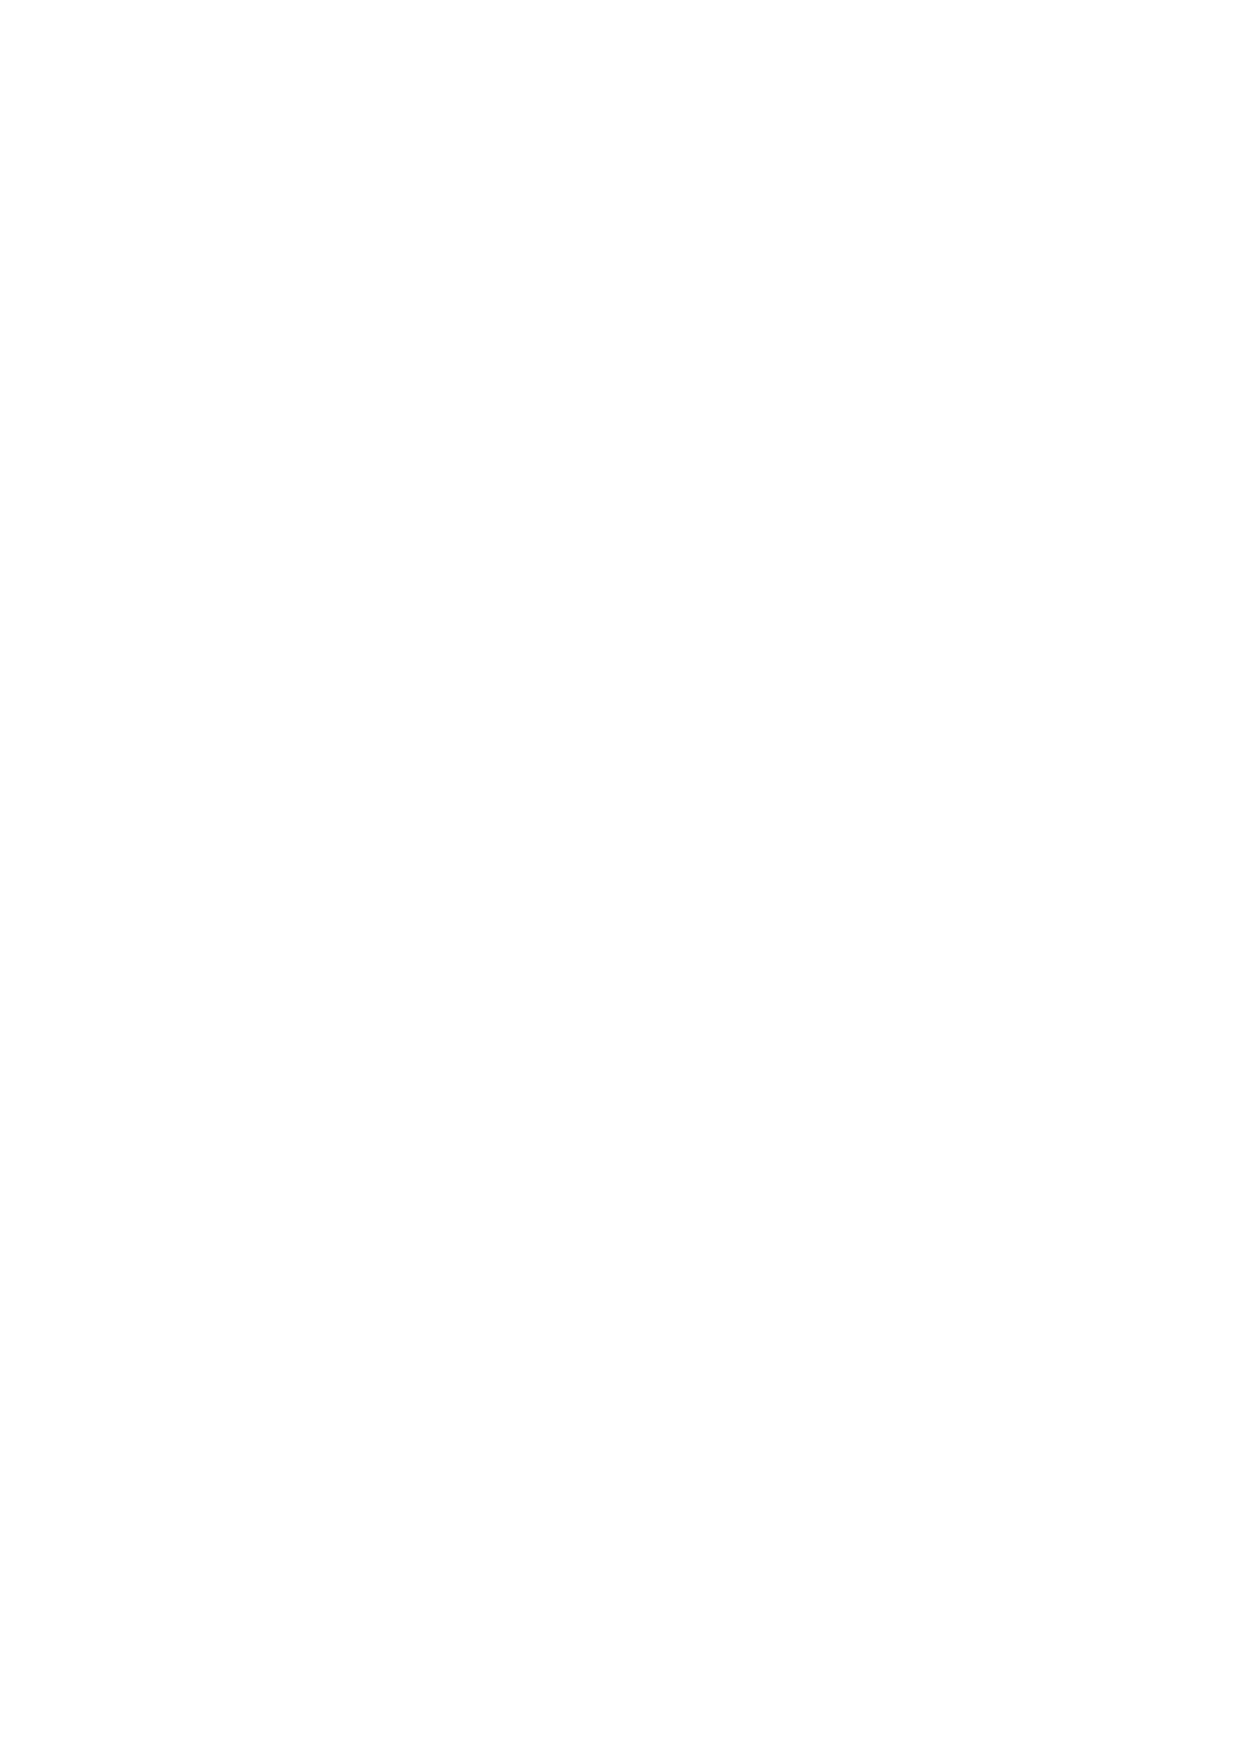
\includepdf{pdf/titel_leer}           	% zum Ausdruck auf die Pappe
}

%---------------------------------------------------------------------------------------------------
% Erstellung von Titelblatt (Seite 2)
% Anwendung:
% \createTitlePage{Art der Arbeit}{Author}{Titel}{Studiengang}{Erstprüfer}{Zweitprüfer}
%---------------------------------------------------------------------------------------------------
\newcommand{\createTitlePage}[7]{
	\thispagestyle{empty}

	\setlength{\TPHorizModule}{1mm}
	\setlength{\TPVertModule}{\TPHorizModule}
	\textblockorigin{0mm}{0mm} % start everything near the top-left corner

	% Name & Titel
	\begin{textblock}{130}(40,63)
		\begin{minipage}[c][5,9cm][t]{13cm}
			\begin{center}
			\linespread{1.2}
			\fontsize{18pt}{18pt}
  		\selectfont
  		#2 \\ \medskip
  		\fontsize{16pt}{16pt}
  		#3
  		\end{center}
		\end{minipage}
	\end{textblock}

	% Infos zur Arbeit und zum Fachbereich
	\begin{textblock}{126}(32,214)
  	\begin{minipage}[t][5,72cm][l]{12,57cm}
    	\fontsize{12pt}{12pt}
    	\selectfont
    	#1 eingereicht im Rahmen der #1prüfung\\
    	im Studiengang #4\\
			am Department Informatik\\
			der Fakultät Technik und Informatik\\
			der Hochschule für Angewandte Wissenschaften Hamburg\\
			\\\
			\\\
			Betreuender Prüfer : #5\\
			Zweitgutachter : #6\\
			\\\
			Abgegeben am \today
  	\end{minipage}
	\end{textblock}
	\	% WICHTIG! Damit wird nach dem Titelblatt eine neue Seite angefangen! Sonst werden Titelblatt &
  	% Danksagung auf eine Seite gedruckt!
}

%---------------------------------------------------------------------------------------------------
% Versicherung über Selbstständigkeit
%---------------------------------------------------------------------------------------------------
\newcommand{\asurency}{
	\chapter*{Versicherung über Selbstständigkeit}
	\vfill
	Hiermit versichere ich, dass ich die vorliegende Arbeit im Sinne der Prü\-fungs\-ord\-nung nach \S 24(5) 		ohne fremde Hilfe selbstständig verfasst und nur die angegebenen Hilfsmittel benutzt habe.
	\vfill
	\begin{tabularx}{\linewidth}{X l X}
	Hamburg, \today	& \qquad \qquad \qquad	& \\
	\cline{1-1}
	\cline{3-3}
	Ort, Datum	& \qquad \qquad \qquad	& Unterschrift \\
	\end{tabularx}
	\vfill
	\vfill
	\vfill
}

%---------------------------------------------------------------------------------------------------
% Fügt ein Wort dem Index zu
%---------------------------------------------------------------------------------------------------
\newcommand{\toIndex}[1]{#1\index{#1}}

%---------------------------------------------------------------------------------------------------
% Dient zum Eintragen folgender Dinge in die Zusammenfassung (Abstract):
%	- Thema
% - Stichworte
% - Kurzfassung
% Benutzung wie folgt:
% \abstractentry{Titel}{Text}
%---------------------------------------------------------------------------------------------------
\newcommand{\abstractentry}[2]{
	\textbf{\large#1}\\
	\nobreakspace
	\begin{tabular}{lp{142mm}}
		\hspace*{7mm} & #2 \\
	\end{tabular}
	\vfill
}

%---------------------------------------------------------------------------------------------------
% Erstellt eine Defintion
% Anwendung: \definition{Die Definition}
%---------------------------------------------------------------------------------------------------
\newcommand{\definition}[1]{
\begin{tabular}[ht]{lp{135mm}}
	\textbf{Def.:} & #1 \\
\end{tabular}
}

%---------------------------------------------------------------------------------------------------
% Erstellt eine Widmung
% Anwendung: \dedication{Wem ist das Schriftstück gewidmet}
%---------------------------------------------------------------------------------------------------
\newcommand{\createDedication}[1]{
	\newpage
	\thispagestyle{empty}
	\begin{tabular}{lp{60mm}}
		\hspace*{100mm} & \itshape\rmfamily#1 \\
	\end{tabular}
	\vfill
}

%---------------------------------------------------------------------------------------------------
% Häufig verwendete Namen mit Literaturverweis und Indexeintrag
%--------------------------------------------------------------------------------------------------
\newcommand{\butrynowski}{Christian Butrynowski\index{Butrynowski, Christian} \citep{Butrynowski:2005}\xspace}
\newcommand{\luepke}{André Lüpke\index{Lüpke, André}\citep{Luepke:2004}\xspace}
\newcommand{\bresch}{Marco Bresch\index{Bresch, Marco} \citep{Bresch:2004}\xspace}


%---------------------------------------------------------------------------------------------------
% Die folgenden Befehle wurden aus der Vorlage von Michael Knop übernommen
%--------------------------------------------------------------------------------------------------
%---------------------------------------------------------------------------------------------------
% Ident
%---------------------------------------------------------------------------------------------------
\newcommand{\ident}[1]{                             % ein Parameter
	\small\ttfamily#1\sffamily\normalsize
}

%---------------------------------------------------------------------------------------------------
% Kürzel
%---------------------------------------------------------------------------------------------------
% Hier sind Makros definiert, die die Eingabe erleichtern sollen. Für korrekte Abstände zwischen
% "z.B." sorgt also ein "z.\,B." (LaTeX-Befehl für kleineren Abstand)
% Schneller schreibt sich das durch das Makro "\zB":

% \newcommand{\zB}{z.\,B.\ }

% Hier ist der Rest aber mit dem Paket xspace verwirklicht. Damit kann
% man bei Bedarf den Abstand mit "\hspace" exakt eingeben. Dann zeigt
% LaTeX keine Toleranz bei den Abkürzungen und macht eben exakt das
% untenstehende.

%\renewcommand{\entryname}{K\"urzel}
%\renewcommand{\descriptionname}{Beschreibung}

\newcommand{\vgl}{vgl.\@\xspace}
\newcommand{\abb}{Abb.\@\xspace}
\newcommand{\zB}{z.\nolinebreak[4]\hspace{0.125em}\nolinebreak[4]B.\@\xspace}
\newcommand{\bzw}{bzw.\@\xspace}
\newcommand{\dahe}{d.\nolinebreak[4]\hspace{0.125em}h.\nolinebreak[4]\@\xspace}
\newcommand{\etc}{etc.\@\xspace}
\newcommand{\bzgl}{bzgl.\@\xspace}
\newcommand{\so}{s.\nolinebreak[4]\hspace{0.125em}\nolinebreak[4]o.\@\xspace}
\newcommand{\iA}{i.\nolinebreak[4]\hspace{0.125em}\nolinebreak[4]A.\@\xspace}
\newcommand{\sa}{s.\nolinebreak[4]\hspace{0.125em}\nolinebreak[4]a.\@\xspace}
\newcommand{\su}{s.\nolinebreak[4]\hspace{0.125em}\nolinebreak[4]u.\@\xspace}
\newcommand{\ua}{u.\nolinebreak[4]\hspace{0.125em}\nolinebreak[4]a.\@\xspace}
\newcommand{\og}{o.\nolinebreak[4]\hspace{0.125em}\nolinebreak[4]g.\@\xspace}

\newcommand{\HAW}{Hochschule für Angewandte Wissenschaften Hamburg\xspace}
\newcommand{\GNU}{GNU\xspace}
\newcommand{\GPL}{\GNU Public License\xspace}

\newcommand{\ACM}{ACM\xspace}
\newcommand{\PDA}{PDA\xspace}


%---------------------------------------------------------------------------------------------------
% Trennung
%---------------------------------------------------------------------------------------------------
%---------------------------------------------------------------------------------------------------
% Trennung
% Hier können alle Wörtertrennungen definiert werden. Die nachfolgenden dienen als Beispiel
% und wurden aus der Vorlage von Michael Knop übernommen.
%---------------------------------------------------------------------------------------------------
\hyphenation{Web-ap-pli-ka-tion Web-ap-pli-ka-tio-nen Web-an-wen-dung Web-an-wen-dung-en My-SQL Kon-text-in-for-ma-ti-onen}

%---------------------------------------------------------------------------------------------------
% Anpassung der Parameter, die TeX bei der Berechnung der Zeilenumbrüche verwendet:
%---------------------------------------------------------------------------------------------------
\tolerance 1414
\hbadness 1414
\emergencystretch 1.5em
\hfuzz 0.3pt
\widowpenalty=10000
\vfuzz \hfuzz
\raggedbottom
 % Die stilistischen Parameter

\date{31.08.2012}
%---------------------------------------------------------------------------------------------------
% Anfang des Schriftstücks
%---------------------------------------------------------------------------------------------------
\begin{document}

%---------------------------------------------------------------------------------------------------
% Erstellen des Deck- und des Titelblatts
%---------------------------------------------------------------------------------------------------
\createCover{Erweiterung des Routing-Atlas\\
WiSe 2011/2012 - 31.08.2012} % Art der Arbeit
{Andreas Krohn} % Author
{Ausarbeitung: Related Work (AW2)} % Title

%---------------------------------------------------------------------------------------------------
% Zusammenfassung}
%---------------------------------------------------------------------------------------------------
% %---------------------------------------------------------------------------------------------------
% Zusammenfassung
%---------------------------------------------------------------------------------------------------
\newpage
\thispagestyle{empty}
\subsection*{Martin Mustermann}
\abstractentry{Thema der Bachelorarbeit}{Mein Titel der Arbeit: Sollte kurz und interessant klingen und nicht die gesamte Aufgabenstellung und Abgrenzungen beinhalten.}
\abstractentry{Stichworte}{...die wichtigsten Stichwörter}
\abstractentry{Kurzzusammenfassung}{
In dieser Arbeit wurde....
}

\selectlanguage{english}
\subsection*{Martin Mustermann}
\abstractentry{Title of the paper}{My title of the paper: Should sound short and interesting and should not contain the complete type of problem and delimitations.}
\abstractentry{Keywords}{...the most important keywords}
\abstractentry{Abstract}{
In this paper...
}
\selectlanguage{ngerman}


%---------------------------------------------------------------------------------------------------
% Verzeichnisse
%---------------------------------------------------------------------------------------------------
\tableofcontents % Inhaltsverzeichnis
% \listoftables % Tabellenverzeichnis
% \listoffigures % Abbildungsverzeichnis

%---------------------------------------------------------------------------------------------------
% Einführung
%---------------------------------------------------------------------------------------------------
\newpage
%\part{Anfang}
%\abstractentry{Kurzzusammenfassung}{KURZE BIS 5 zeilige Zusammenfassung}

\section{Einführung}

Die Bedeutung des Internets nimmt in den letzten Jahren stetig zu.
Kommunikation, Verwaltung und Abwicklung von Geschäften verlagern sich zunehmend ins Internet.
Gleichzeitig wachsen die Bestrebungen seitens der Politik und Unternehmen Einfluss auszuüben - sei es zur Durchsetzung von Gesetzen oder zur Gewinnmaximierung.
Angesichts dieser Tatsache ist es interessant zu analysieren, welche Akteure die Daten beispielsweise auf dem Weg zwischen Geschäftspartnern oder zwischen einer Behörde und Bürgern traversieren. %Da das Internet diese Informationen jedoch nicht "`freiwillig"' .. hmm ne..
Um dieses Wissen zu erlangen, sind Topologieanalysen nötig, wie sie das Routing-Atlas Projekt durchführt.

Der Bereich Topologieanalyse wird von weiteren Arbeitsgruppen bearbeitet.
Teils werden die dabei entstehenden Resultate vom Routing-Atlas Projekt direkt genutzt, teils werden eigene Wege beschritten.
In der vorliegenden Ausarbeitung wird eine Auswahl vergleichbarer Arbeiten vorgestellt.
Dabei wird grob zwischen den Bereichen Datensammlung und Modellierung unterschieden.
Abschnitt~\ref{sec:datenquellen} stellt Arbeiten im Bereich Datensammlung vor, Abschnitt~\ref{sec:modellierung} Arbeiten im Bereich Modellierung.

% In dieser Ausarbeitung wird der Routing-Atlas sowie die geplanten Änderungen vorgestellt.

% In Abschnitt~\ref{sec:atlas} wird zunächst auf die bereits vorhandenen Schritte und Datenquellen zur Erstellung des Routing-Atlas eingegangen.
% Abschnitt~\ref{sec:zielsetzung} umreißt die Zielsetzung, deren Hauptbestandteil - Ersatz einer externen, nicht mehr aktualisierten Datenquelle - in Abschnitt~\ref{sec:konzept} erläutert wird.
% Abschnitt~\ref{sec:challenge} zeigt, welche Herausforderungen erwartet werden.
% Den Abschluss bilden der Ausblick auf weitere Ausbaumöglichkeiten des Routing-Atlas in Abschnitt~\ref{sec:ausblick} und die Zusammenfassung in Abschnitt~\ref{sec:schluss}


\section{Routing-Atlas}\label{sec:routingatlas}

Der Routing-Atlas ist ein Projekt der FU Berlin und der HAW Hamburg in Zusammenarbeit mit dem Bundesamt für Sicherheit in der Informationstechnik (BSI), \vgl \cite{wsbh-envgi-12}.
Das Projekt will landesspezifische Bestandteile des Internets identifizieren, klassifizieren und visualisieren.
Diese Daten sollen vielfältige Fragestellungen beantworten helfen.
Zum Beispiel nach der Abhängigkeit der Länder untereinander, nach der Abgeschlossenheit der Infrastruktur innerhalb eines Landes und nach der Bedeutung einzelner Akteure.

Erster Schritt des Projektes ist es eine möglichst korrekte Zuordnung von Bestandteilen des Internets zu Ländern durchzuführen.
Als Beispiel dient hierbei Deutschland.
Gegenüber vorherigen Arbeiten zum Beispiel von Josh Karlin et~al.~\cite{0903.3218v1} wird die Zuordnung nicht ausgehend von IP-Präfixen sondern feingranularer auf Ebene von IP-Adressblöcken vorgenommen.
Die Zuordnung der IP-Adressblöcke zu einem Land geschieht basierend auf Daten der zuständigen RIR - für Deutschland die RIPE~\cite{RIPE} - in einem mehrstufigen Verfahren.
Als Kandidaten werden jene Adressblöcke betrachtet, deren \texttt{country} Attribut "`DE"' oder "`EU"' lautet.
Zu Verfizierung der "`DE"' und zur Identifizierung weiterer "`EU"' als deutsch werden nun Kontaktinformationen zu den Adressblöcken ausgewertet und gegen eine Liste von Synonymen, geographischen Namen und Schlagworten abgeglichen.
Die so als deutsch identifizierten Adressblöcke werden nun zu IP-Präfixen und anschließend zu ASen aufgelöst.

Die einem Land zugehörigen ASe werden nach den Aspekten Hierarchie und Branche klassifiziert.
Die Hierarchie gibt an, welche Bedeutung ein AS für das Routing hat und wird aus Daten von Beichuan Zhang et~al.~\cite{Zhang:2005:CIA:1052812.1052825} übernommen.
Die Branche ordnet ein AS einem der folgenden Sektoren zu:
\begin{center}
  \begin{tabular}[h]{ll}
    \hline
    Behören, Verwaltung und Justiz & I\&K: Software- und Systeme \\
    Energie & Industrie (Produzierendes Gewerbe) \\
    Finanz-, Geld- und Versicherungswesen & Medizinwesen \\
    Gefahrenstoffe & Presse, Medien, Verlage \\
    I\&K: Internet Peering Points & Transport und Verkehr \\
    I\&K: ISPs (ohne Endkunden-Zugang),\\
    Internet Infrastruktur & Wissenschaft, Forschung \& Kultur \\
    I\&K: Access Provider & Sonstiges \\
    \hline
  \end{tabular}
\end{center}
Die Branchenzuordnung geschieht basierend auf einer Liste von Schlagworten, die mit den in der RIPE DB vorhandenen Metainformationen (Name, Beschreibung und Adressfeldern) der ASen verglichen wird.

Für die identifizierten und klassifizierten ASe wird der umspannende Routing-Graph durch Traversieren der verbindenden Pfade zwischen allen Paaren der als deutsch identifizierten ASe ermittelt.
Dazu wird die shortest path matrix von Winter (\vgl Abschnitt~\ref{subsec:winter}) genutzt.
Erwartungsgemäß werden damit bisher nicht betrachtete verbindende ASe anderer Länder aufgenommen.

Der so entstandene, mit den Eigenschaften Land, Hierarchie und Sektor annotierte Graph wird anschließend visualisiert.
Um dabei Aussagekraft und Übersichtlichkeit zu steigern, wird der Graph nach unterschiedlichen Aspekten vorgefiltert und auf verschiedene Arten visualisiert.
So werden zum Beispiel die ASe zweier Sektoren gegenübergestellt und durch die verbindenden, nach Hierarchie angeordneten ASe ergänzt.
Weitere Darstellungen zeigen ASe eines Sektoren inklusive verbindender ASe wahlweise hierarchisch in Schichten oder Ringen angeordnet oder unsortiert.
Die Farbe der Knoten steht dabei für den Sektor des zugehörigen AS.
Abbildung~\ref{fig:asgraph_cat10} auf Seite~\pageref{fig:asgraph_cat10} zeigt die Autonomen Systeme des Sektors "`Wissenschaft, Forschung \& Kultur (F\&E)"' in einem hierarchischen Kreisdiagramm.
Die Position eines AS in diesem Diagramm bedeutet, dass es in seiner topologischen Bedeutung (von innen nach außen) Tier 1, Large ISP, Small ISP und Stub zuzuordnen ist.

\begin{figure}
  \begin{center}
  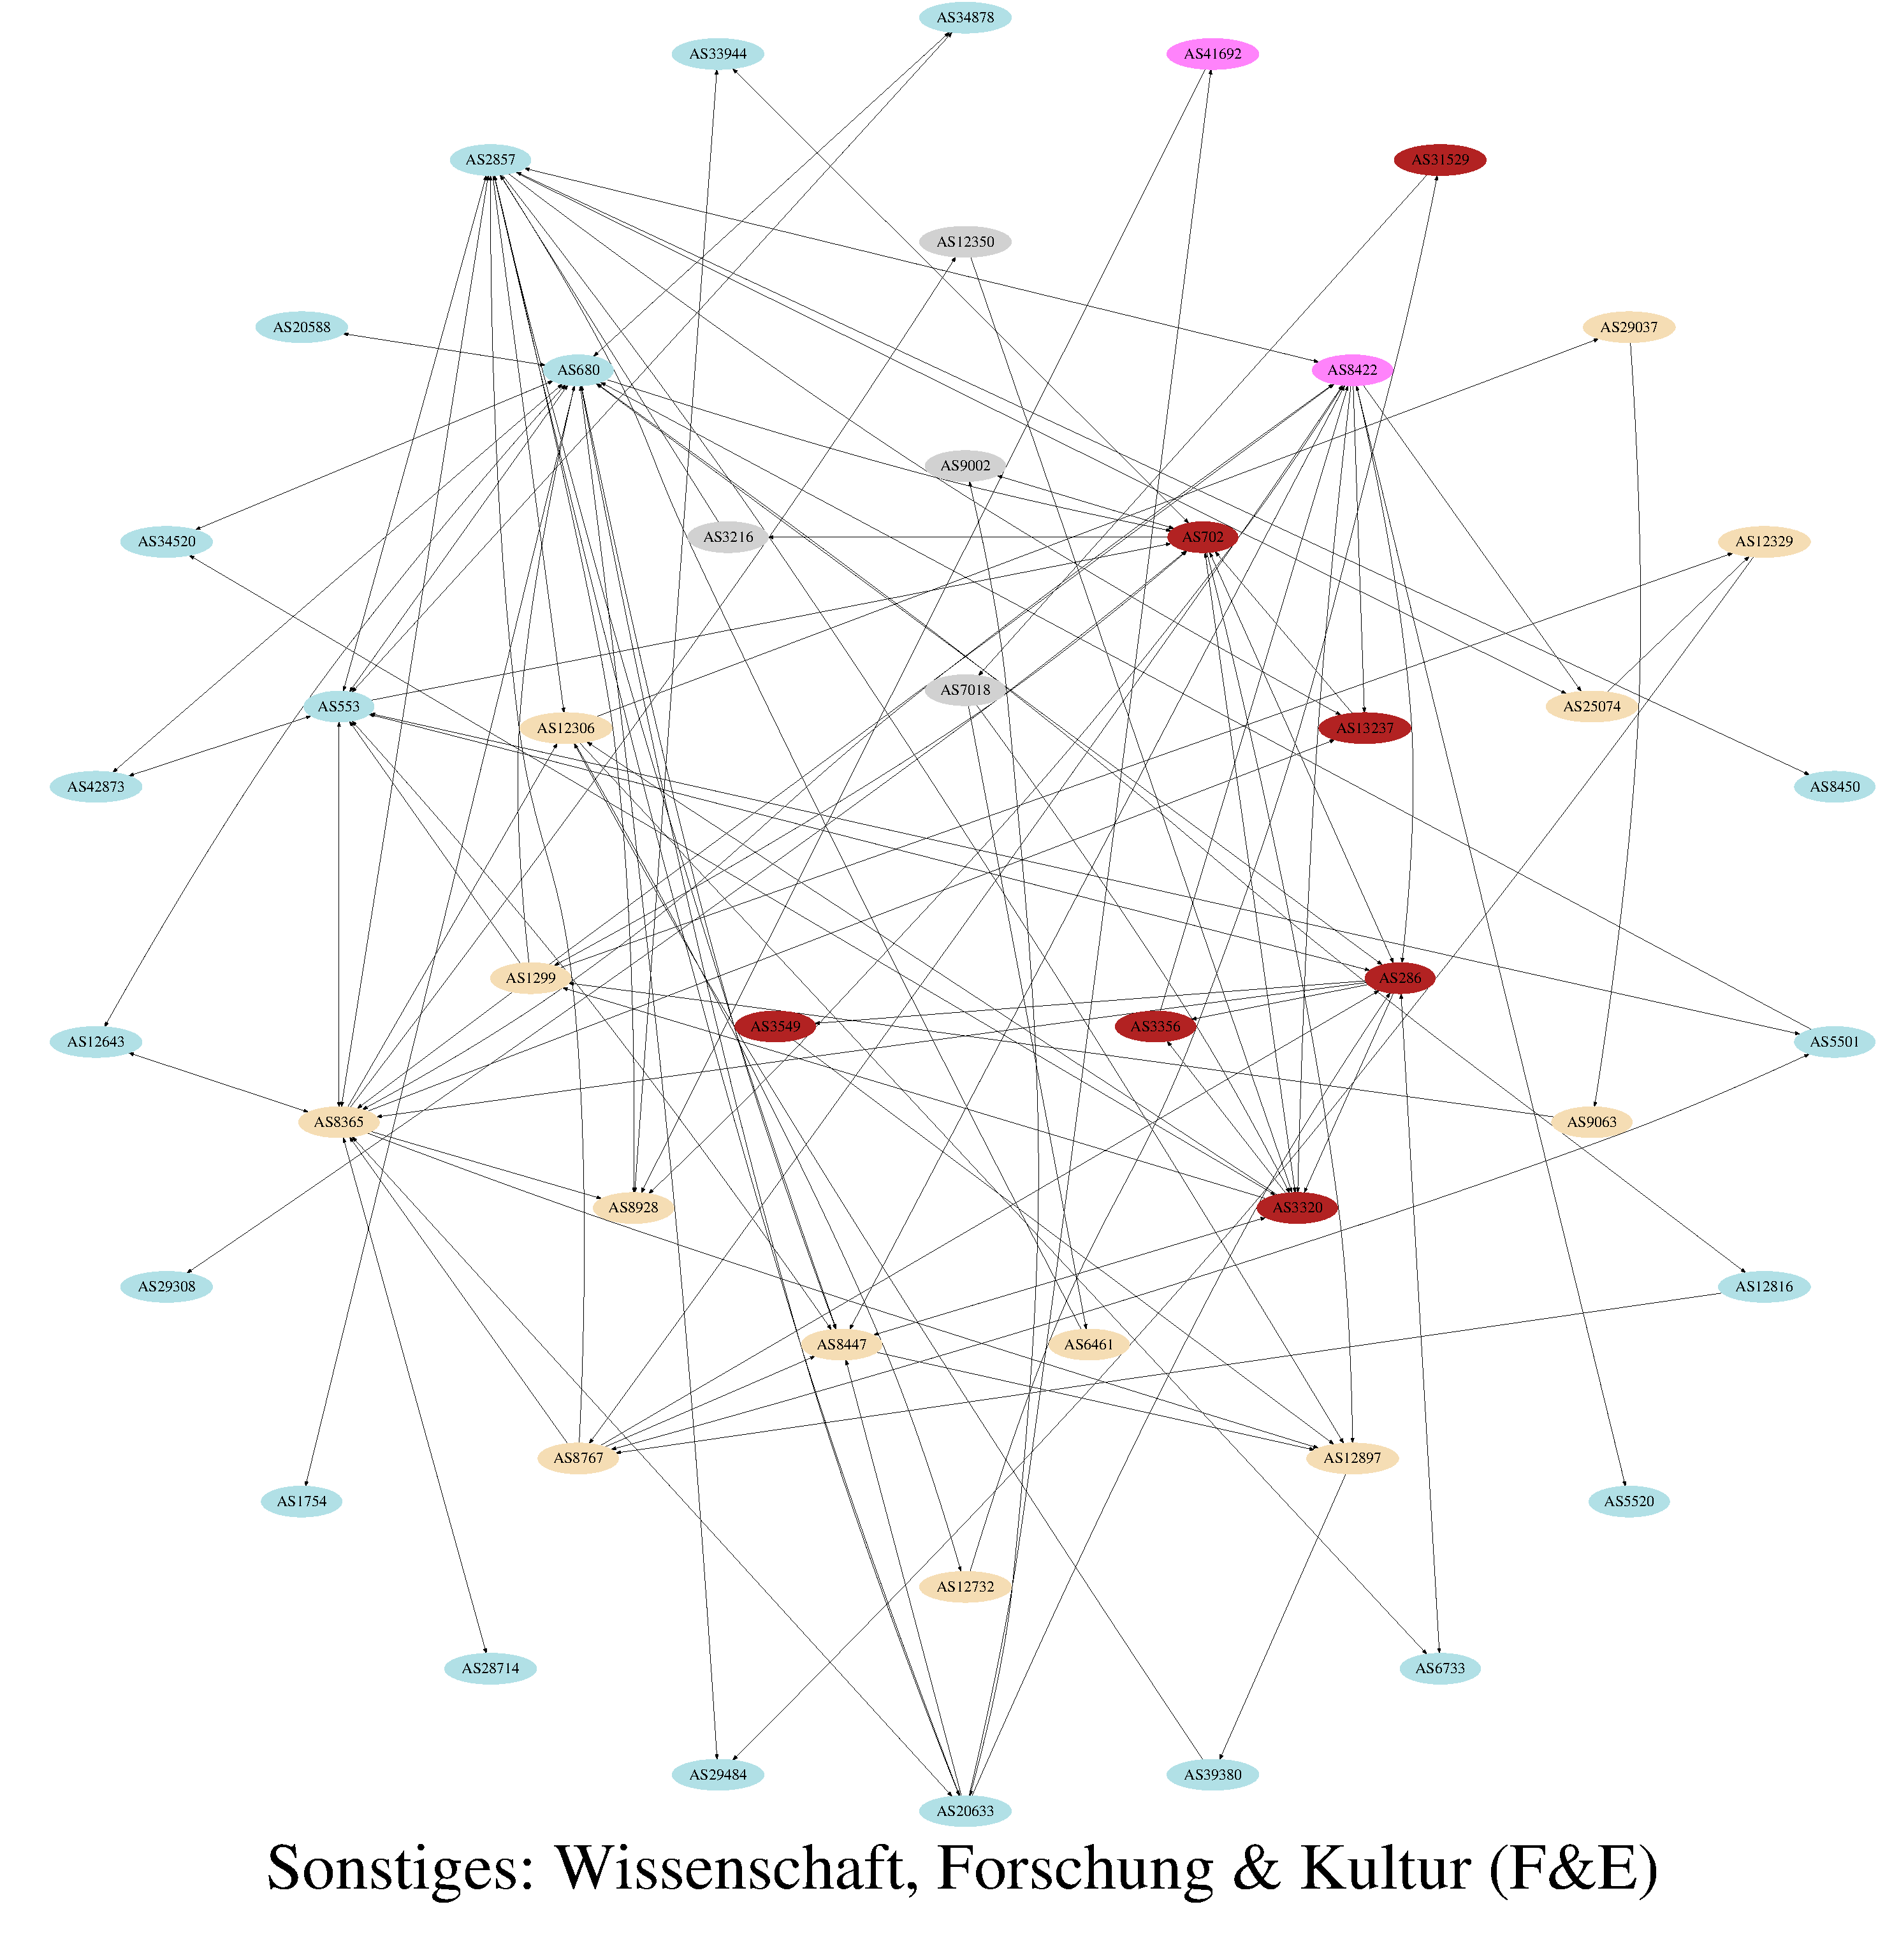
\includegraphics[width=0.55\textwidth]{asgraph_cat10-pos}
  \caption{Hierarchisches Kreismodell - Entnommen aus~\cite{swbh-rsved-11}} \label{fig:asgraph_cat10}
  \end{center}
\end{figure}

\section{Datenquellen}\label{sec:datenquellen}

Das Internet ist eine Menge untereinander verbundener Netze, den autonomen
Systemen (ASe). Die Verwaltung dieser Netze obliegt jeweils dem Besitzer. Es
gibt nicht eine zentrale Verwaltung, die über sämtliche Informationen verfügt.
Diese Aufgabe erfüllen lokale Registries (RIRs), bei denen beispielsweise eine
ASN beantragt werden kann. Die Existenz und einige Informationen zu einem AS
lassen sich bei den RIRs prüfen. Die Existenz und Konditionen der Verbindung
zweier ASe wird nicht erfasst, sondern lässt sich aus aktiven Messungen und der
Auswertung von Routingtabellen mehr oder weniger präzise herleiten. Die
Information, ob ASe miteinander verbunden sind und welcher Art diese Verbindung
ist ermöglicht die Berechnung der Topologie des Internets auf AS Ebene.

Als Beispiel für das passive Methoden der Datensammlung dient hier die Arbeit
von Beichuan Zhang et\ al., für aktive Methoden der Beitrag von Brice Augusting
et\ al..

\subsection{Collecting the Internet AS-level Topology~\cite{Zhang:2005:CIA:1052812.1052825}}

Sammeln Daten und stellen sie täglich aktualisiert bereit\footnote{\url{http://irl.cs.ucla.edu/topology/}}


\subsection{IXPs: Mapped?~\cite{Augustin:2009:IM:1644893.1644934}}

Wollen Peerings an IXPs finden, indem sie traceroutes "durch" IXPs aufrufen.

\section{Modellierung}\label{sec:modellierung}

Alleine aus der Existenz eines Links zwischen ASen lässt sich nicht abschätzen, ob und für welchen Datenverkehr der Link benutzt wird.
Es erfordert vielmehr die Bildung eines Modells, das das policy based routing von BGP nachbildet.
Ein solches Modell klassifiziert die Art der Beziehung zwischen zwei ASen.
Basierend auf dieser Klassifizierung kann hergeleitet werden, welche Pfade möglich sind und verwendet werden.
Dabei wird von einem weitesgehend hierarchischem Aufbau AS Topologie ausgegangen.
Die zentraleren Transit oder Tier-1 ASe leiten hierbei Daten für die kleineren ASe weiter.
Kleinere ASe bieten dagegen keinen Transit für größere ASe an.
Dieses Konzept bezeichnet man als das Valley-free Routing.
Über ein Modell sollen rohe Daten wie BGP Tabellen um Klassifizierungen erweitert werden um auf Basis des so entstehenden attributierten AS-Graphen Analysen ausführen zu können.

\subsection{On Inferring Autonomous System Relationships in the Internet}
Grundlegende und viel beachtete Arbeit im Bereich der Klassifizierung von AS Beziehungen hat Lixin Gao mit der im folgenden Abschnitt vorgestellten Arbeit geleistet~\cite{Gao:2001:IAS:504611.504616}.
Das Prinzip des valley-free Routings führt zu der Erkenntnis, dass Verbindung im Internet nicht Erreichbarkeit bedeuten muss.
Der Transport von Daten folgt policies, die über das BGP Protokoll implementiert werden.
Ziel der Arbeit von Lixin Gao ist es die Kanten eines AS Graphen zu annotieren, also die Links zu klassifizieren.
Die Klassen sind dabei:
\begin{itemize}
  \item customer-provider
  \item peering
  \item sibling
\end{itemize}
Da die Geschäftsbeziehung mehrerer ASe Ursache für die Gestaltung von BGP tables, nicht aber deren Bestandteil sind, wird diese Information über eine Heuristik hergeleitet.

\subsubsection{Vorgehensweise}
Für eine Menge von BGP Tabellen wird der Verzweigungsgrad der ASe bestimmt, der später als Indiz für die Größe des ASes verwendet wird.
In jedem AS Pfad in den BGP Tabellen wird nun das größte AS gesucht.
Die Links im Pfad bis zum größten AS (uphill) werden als Nutzer von Transit, die Links ab dem größten AS (downhill) als Anbieter von Transit markiert.
In einer weiteren Phase geschieht nun die eigentliche Klassifizierung.
Ist ein Paar aus ASen in beide Richtungen als Transit markiert, so gehört dieser Link in die Klasse "`sibling"'.
Ist ein Paar aus ASen Nutzer von Transit aber selten oder nie Anbieter, ist der Link ein "`customer-provider"'-Link, überwiegt die Anbieterrolle "`provider-customer"'.

\subsubsection{Beitrag}

\subsection{Modeling the Internet Routing Topology - in less than 24h}\label{subsec:winter}
Der attributierte AS-Graph liefert Informationen über Existenz und Art der Verbindung der ASe.
Der Weg, den der Datenpakete zwischen zwei ASen traversiert, lässt sich hieraus jedoch nicht ablesen.
Rolf Winter (damals NEC Labs Europe, jetzt Hochschule Augsburg) beschreibt in seinem Artikel "`Modeling the Internet Routing Topology - in less than 24h"'~\cite{conf/pads/Winter09} einen Ansatz, die kürzesten Wege zwischen allen AS-Paaren unter Berücksichtigung eines Modells von BGP zu berechnen.

\subsubsection{Vorgehensweise}
....


\subsubsection{Beitrag}
....

\section{Ausblick}\label{sec:ausblick}
Die laufende Schaffung eines Ersatz für die nicht mehr aktualisierte shortest path matrix von Rolf Winter und die Automatisierung der vorhandenen Toolchain des Routing Atlas wird die regelmäßige öffentliche Bereitstellung der länderspezifischen Auswertungen ermöglichen.
Weiterhin bietet der Bereich der in Abschnitt~\ref{subsec:ixps} vorgestellten aktiven Messungen interessante Möglichkeiten.
Es besteht Kontakt zu den Betreibern eines IXPs, sodass Messungen durchgeführt werden können mit denen zum Beispiel verwendete Topologiedaten nachvollzogen und verifiziert werden können.
Weiterhin ist die Ergänzung der verwendeten Topologiedaten um eigene mittels traceroute erhobene Daten oder um die von Augustin et~al. zu prüfen.
% Schaffung von Ersatz für next hop matrix: bald.
% Experimente mit traceroute in/an IXP: Validierung \& Nachvollziehen der UCLA Daten; Bei Eignung Erweiterung der UCLA-Daten um weitere Peerings.


%---------------------------------------------------------------------------------------------------
% Schluss
%---------------------------------------------------------------------------------------------------
\section{Zusammenfassung}\label{sec:schluss}

In dieser Ausarbeitung wurde der Routing-Atlas in seiner derzeitigen Form vorgestellt.
Weiterhin wurde Winters Konzept zur Generierung von shortest path und next hop matrix, sowie die geplanten Anpassungen um diese Generierung in die Toolchain des Routing-Atlas zu integrieren, gezeigt.

Die dabei erwarteten Herausforderungen und mögliche Abhilfen wurden aufgezeigt.

Der Ausblick zeigt weitere Betätigungsfelder auf, die nach der Lösung der shortest path und next hop matrix Problematik in Angriff genommen werden sollen.
\newpage


%---------------------------------------------------------------------------------------------------
% Literaturverzeichnis
%---------------------------------------------------------------------------------------------------
%\bibliographystyle{dinat} % Anpassung an deutsche Zitierweise: Alphabetische Sortierung, Abkürzungen
%\bibliographystyle{unsrt}
\bibliographystyle{IEEEtran} % dinat.bst fehlt, kein format für @ONLINE, gefällt mir so irgendwie besser..
\bibliography{literatur/literatur2} % Literaturverzeichnis

%---------------------------------------------------------------------------------------------------
% Ende des Schriftstücks
%---------------------------------------------------------------------------------------------------
\end{document}
